\documentclass[a4paper, 12pt]{report}
\usepackage[pdftex]{graphicx}
\usepackage[autostyle]{csquotes}
\usepackage[backend=bibtex,style=numeric,sorting=none]{biblatex}
\usepackage{caption}
\usepackage{subcaption} % for subfigure
\usepackage{hyperref}
\usepackage{amssymb}
\usepackage{tabularx}
\usepackage{multicol}
\usepackage{algpseudocode}
\usepackage{amsthm} % for theorem
\usepackage{algorithm}
\addbibresource{bibliography}

\theoremstyle{plain}
\newtheorem{thm}{Theorem}[chapter] % reset theorem numbering for each chapter

\theoremstyle{definition}
\newtheorem{defn}[thm]{Definition} % definition numbers are dependent on theorem numbers
\newtheorem{exmp}[thm]{Example} % same for example numbers

\begin{document}
\pagenumbering{roman}
\begin{titlepage}
\begin{center}

{\Huge \bfseries
Virtual Multi-Tenant Networks Simulator \\
using Software Defined Networks\\
}~\\[1cm]

% The '~' is needed because \\ only works if a paragraph has started.

{\large \bfseries
B.Tech. Project 1st Stage Report
}~\\[0.40cm]

{
Submitted in partial fulfilment of the requirements for the degree of
}~\\[0.20cm]

{\large \bfseries
Bachelor of Technology (Honors)
}\\[2.75cm]
\end{center}

\begin{multicols}{2}
\begin{flushleft}
{\large
\textit{Student:} \\
\textbf{Kausik Subramanian	} \\
\textbf{Roll No: 110050003}
}
\end{flushleft}
\columnbreak
\begin{flushright}
{\large
\textit{Guide:} \\
\textbf{Purushottam Kulkarni}
}
\end{flushright}
\end{multicols}

\vfill

\begin{center}

\includegraphics[width=4cm]{Figures/iitbblack.jpg}~\\[1cm]

{\large
Department of Computer Science and Engineering\\
Indian Institute of Technology Bombay\\
Mumbai 400076, India\\
}

\end{center}
\end{titlepage}
\chapter*{}
\begin{center}
\textbf{Abstract}
\end{center}
Abstract
\addcontentsline{toc}{chapter}{Abstract}
\begin{center}
{\large \bfseries
Acknowledgement
}~\\[1cm]
\end{center}
\begin{flushleft}
{
I wish to express my sincere gratitude and indebtedness to my guide, \\Purushottam Kulkarni and Umesh Bellur for their constant support and guidance throughout the project. I am also indebted to Martin Casado, whose talk on Software defined Networks at IIT Bombay inspired me to pursue research in the field. 
}~\\[1.5cm]
{
Kausik Subramanian\\
B.Tech. IV\\
CSE, IIT Bombay
}
\end{flushleft}

\tableofcontents
\pagenumbering{arabic}
\chapter{Introduction}

Introduction
\chapter{System Design}
POXVine consists of three main components.
\begin{itemize}
	\item The \emph{host mapper} is responsible to map the virtual network entities (hosts and switches) onto the physical topology. This mapping can be done based on different heuristics, so POXVine allows you to customize the host mapper. We have developed a host mapper \emph{MinSwitchMapper}, which tries to minimize the number of \emph{physical switches} which contain rules to the virtual topology.
	
	\item The \emph{network Mapper} is an application built over the \emph{POX} controller which uses the \emph{virtual-to-physical} mappings to add the required routing OpenFlow rules on the mininet switches, so that the virtual hosts can talk to one other. Another important design consideration is that the \emph{virtual network abstraction} must be preserved, that is, if a packet is to flow across a route in the virtual topology, on the physical topology, it must traverse the virtual network entities in the same order.
	
	\item The \emph{Mininet} infrastructure is used to emulate the physical network topology and the virtual hosts which are connected to the emulated physical switches (according to the \emph{virtual-to-physical}) mappings). 	
\end{itemize}  
I explain the individual components in the coming sections.


\begin{figure}
	\noindent
	\makebox[\textwidth]{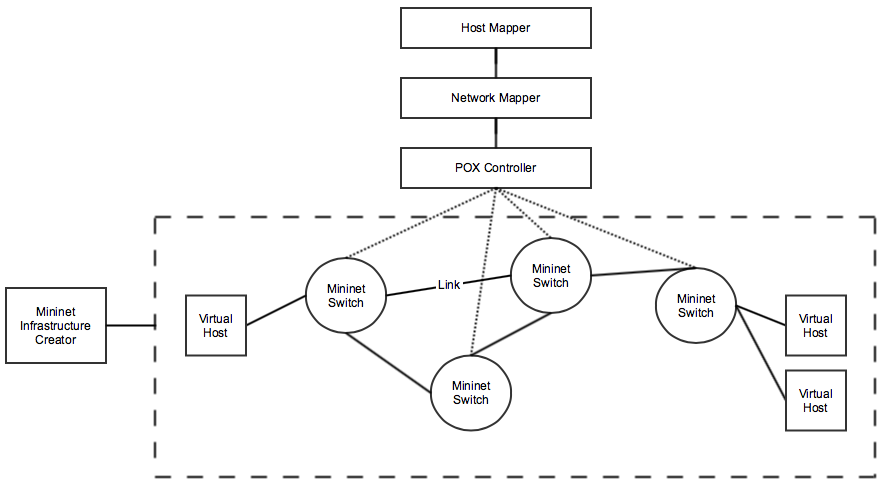
\includegraphics[width=17cm]{Figures/poxvine.png}}%
	\caption{POXVine Architecture}
\end{figure}

\section{MinSwitchMapper}
The host mapper module is responsible for finding the \emph{virtual-to-physical} mappings of the virtual network entities, i.e on which physical hosts, the virtual hosts and switches are placed. This mapping can be done according to various considerations, like \emph{maximizing number of virtual hosts, minimizing the number of switches mapped to a virtual topology, greedy host allocation, providing bandwidth guarantees etc.} \\
All the virtual network entities are mapped to physical hosts, which are connected by the physical network topology. Consider the network graph which is formed by using only the switches and links that are required to connect all the physical hosts (we use the shortest path between two hosts in the network graph). Figure 2.2 demonstrates an example of such a graph. 
\begin{figure}
	\noindent
	\makebox[\textwidth]{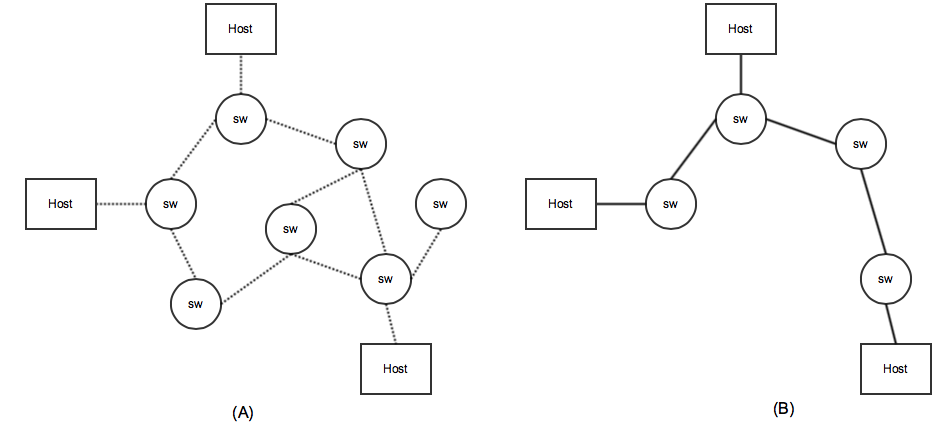
\includegraphics[width=17cm]{Figures/networkg.png}}%
	\caption{POXVine Architecture}
\end{figure}
\\
We have developed \emph{MinSwitchMapper}, which minimises the diameter of the network graph connecting the hosts of the virtual topology, The basis for this heuristic is that the traffic of this tenant's hosts are confined to the \emph{smallest portion} in the physical topology. This also minimises the number of switches where rules regarding this virtual topology is installed, thus increasing the number of tenants we can accomodate in POXVine (provided the physical host capacity is not insufficient)

\section{NetworkMapper}
The \emph{NetworkMapper} module is an application built on top of the POX controller. The role of the NetworkMapper is to use the \emph{virtual-to-physical mappings} generated by the host mapper module and add the required routing rules on the mininet switches for the virtual hosts of a tenant. One important design decision is that the NetworkMapper preserves the \emph{virtual network abstraction}. Let us suppose there are two virtual hosts \emph{v1} and \emph{v2}, connected by a path of two switches \emph{s1} and \emph{s2}, i.e $v1 \rightarrow s1 \rightarrow s2 \rightarrow v2 $.  Irrespective of the mapping, the Network Mapper must add the rules such that traffic from $v1 \rightarrow v2 $ must traverse through $s1$, $s2 $ and $v2$ in that order. 

\subsection{Route Tagging}




 


\chapter{Future Work}
Future Work

\pagenumbering{roman}
\printbibliography[heading=bibintoc]

\end{document}